\section{Software} \label{sec: software}
Describes the used software for the project as well as contains installation guide and version numbers.

\subsection{Software Tools}\label{subsec: software_tools}
Used for documentation is 
\begin{enumerate}[(a)]%for capital roman numbers.
	\item Git, GitHub is used to make backups and commit histories.
	used to make back ups and commit stages of your work.
	\item \LaTeX is the format used to describe the document.
	\item MiK\TeX \cite{MikTex} Consol is a package management system.
	\item \TeX Studio \cite{TexStudio} is an \LaTeX text editor.
	\item Mendeley \cite{Mendeley} reference management software with chrome plug in.
	\item Pandoc is used for Markdown to Latex conversion.	
	
\end{enumerate}

\subsection{Git, GitHub}\label{subsec: install_git}
\href{https://git-scm.com/downloads}{Git} is a fast-version-control tool that  allows the engineer to jump back to any commit that he made. It is available on the three major operating systems Windows, Mac OS X, and Linux/Unix. For Windows there is an additional benefit git comes with a built in Linux/Unix bash terminal so that Linux/Unix commands can be used on Windows and is called Git Bash.


Initializing a git repository in an existing folder locale:
\begin{lstlisting}[language=bash,caption={Initializing a git repository},label=lst: git init]
$ git init
$ git add README.md
$ git commit -m "first commit"
$ git remote add origin https://github.com/userName/repositoryName.git
$ git push -u origin master
\end{lstlisting}
...or cloning an existing repository from GitHub a git repository in an existing folder locale:
\begin{lstlisting}[language=bash,caption={Clone git repository},label=lst: git clone]
$ git clone https://github.com/userName/repositoryName.git
\end{lstlisting}
…or push an existing repository from the command line
\begin{lstlisting}[language=bash,caption={Remote git repository on GitHub},label=lst: git remote]
$ git remote add origin https://github.com/haringd/GeocalculatoriOSHW7.git
$ git push -u origin master
\end{lstlisting}
…or most common git commands used in the command line
\begin{lstlisting}[language=bash,caption={git common commands},label=lst:git common]
$ git pull
$ git status
$ git add .
$ git commit -m "Your commit text"
$ git push

$ git log
$ git checkout <commit>
\end{lstlisting}

In case there was a careless day and a too big file was committed.
% https://stackoverflow.com/questions/2100907/how-to-remove-delete-a-large-file-from-commit-history-in-git-repository
\begin{lstlisting}[language=bash,caption={git bash find files larger then 99MB},label=lst:git common]
$ find . -size +99M -exec ls -lh {} \+
\end{lstlisting}
\begin{lstlisting}[language=bash,caption={git delete files from history which are larger then 99MB},label=lst:git common]
$ git filter-branch --prune-empty -f --index-filter "git rm --cached -f --ignore-unmatch Project2015/simulations/LTC3878_EMC_Project_v2.raw"           
\end{lstlisting}



\subsection{Install \LaTeX}\label{subsec: install_latex}
\subsubsection{Install MiKTeX}\label{subsubsec: install_miktex}
\href{https://miktex.org/}{MiKTeX} provides package management for \LaTeX that handles most packages used for documentation.  

\subsubsection{Install TexStudio}\label{subsubsec: install_texstudio}
\href{https://www.texstudio.org/}{TexStudio} is a convenient front end to edit and write \LaTeX syntax. Like most IDEs it provides auto-completion (ctrl + space). It also provides compiler and build system to convert \LaTeX into a PDF format. Furthermore it integrates easy into git which makes it easier to collaborate in a team.

\subsection{TexStudio Hints}\label{subsec: texstudio_hints}
\subsubsection{Edit Default Language and Dictionary}
As shown in Figure \ref{fig: texstudio_selectDefaultLanguage}, this can be done under Preferences -> Language Checking.
\begin{figure}[ht]
	\centering
	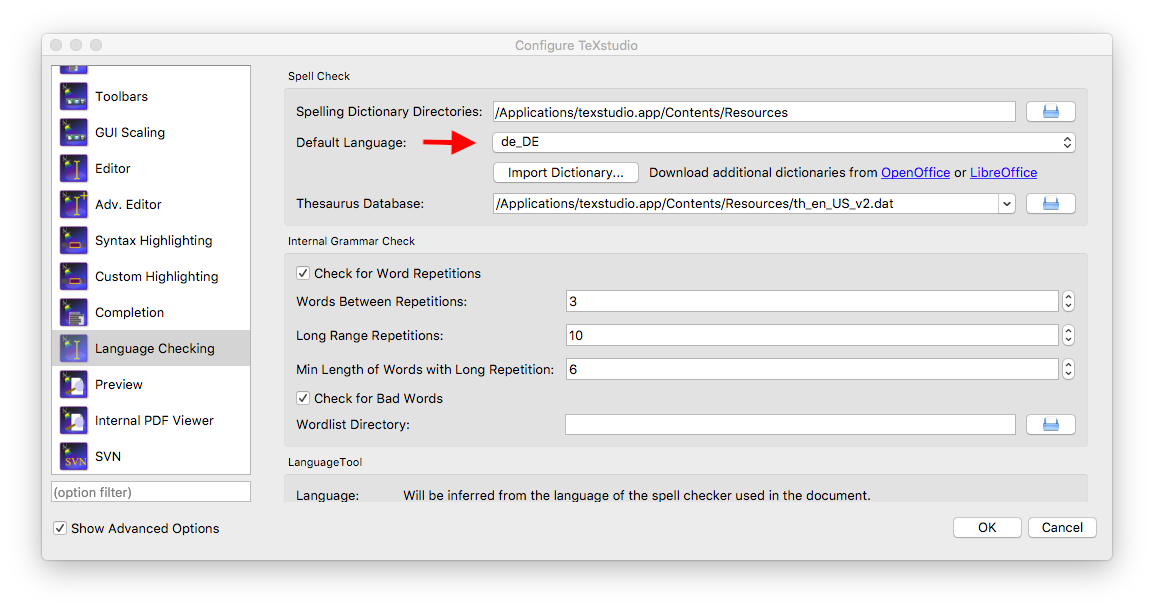
\includegraphics[width=400px ]{02_images/texstudio_selectDefaultLanguage}
	\caption{Language Settings in TexStudio.}
	\label{fig: texstudio_selectDefaultLanguage}
\end{figure}

\subsubsection{Convert a *.md file into a *.tex file}
Pandoc can be used to convert, with a simple terminal command, a *.md file into a *.tex file. Easiest is to convert the file as pre compiler option which can be added shown in Figure \ref{fig: texstudio_convertMDfiletoTEXfilewithPandoc}. The terminal command is shown in Listing \ref{lst: pandoc_bash_convert_file}

\begin{lstlisting}[language=bash, caption=Terminal command that converts .md to .tex files, label=lst: pandoc_bash_convert_file]
pandoc -f markdown -t latex -o onepage.tex ONEPAGE.md.
\end{lstlisting}

\begin{figure}[H]
	\centering
	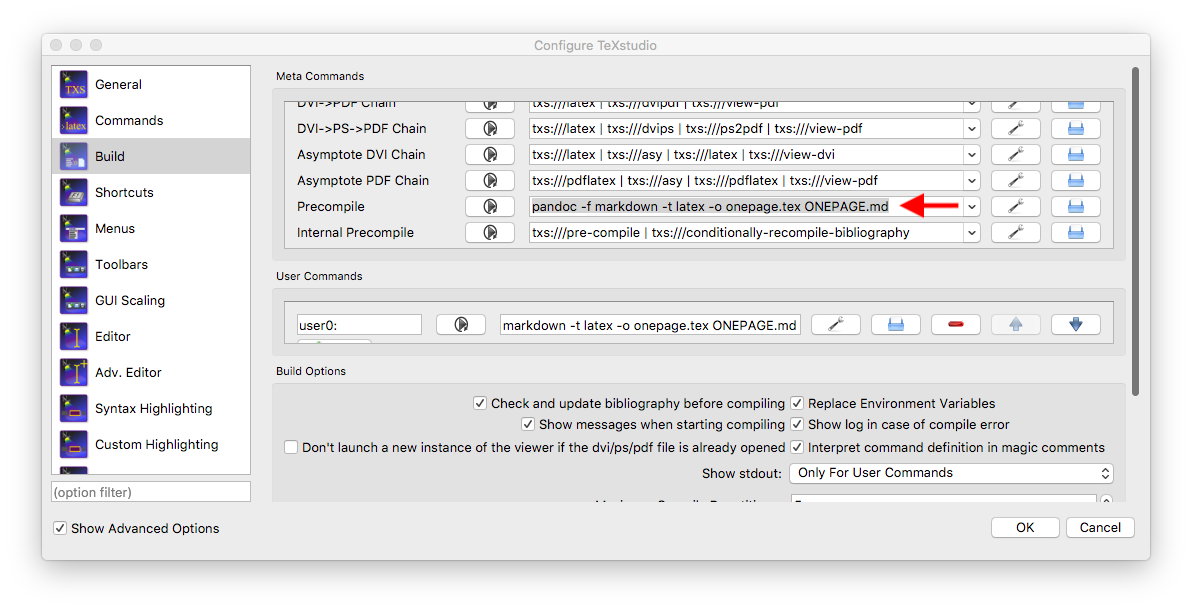
\includegraphics[width=400px ]{02_images/texstudio_convertMDfiletoTEXfilewithPandoc}
	\caption{Language Settings in TexStudio.}
	\label{fig: texstudio_convertMDfiletoTEXfilewithPandoc}
\end{figure}

\subsection{biblatex, make citations with \LaTeX}\label{subsec: Bibtex, make citations with LaTeX}
In order to run the citation properly use the following commands in bash or windows terminal on the file.
\begin{verbatim}
$ pdflatex reportRFTuner
$ biber reportRFTuner
$ pdflatex reportRFTuner
\end{verbatim}
That solves the problem of not showing the citations after editing the *.bib file correctly.

An easy way to handle citations is to use \href{https://www.mendeley.com}{Mendeley} which allows to copy a citation in bibtex format and simply append it to the *.bib file. Just in case you wonder where you got bibtex from it was installed with miktex or texstudio. 

A bibtex file *.bib has the following syntax and is used with the \\cite{Vizmuller1995} \cite{Vizmuller1995} command:

\begin{lstlisting}
@book{Vizmuller1995,
address = {Boston, London},
author = {Vizmuller, Peter},
isbn = {0-89006-754-6},
mendeley-groups = {RF{\_}TUNER RAMI{\_}2018},
pages = {281},
publisher = {Artech House, Inc.},
title = {{RF Design Guide}},
year = {1995}
}
\end{lstlisting}

And an example of a citation with page number \cite[1, 2]{1513092}
\section{File Used and Structure}
Fig. \ref{fig:latexfilestructure} shows the file structure used in this document. The Latex\_Mendeley\_top.tex file is the file that holds the definitions and packages used including the text body. The sections where the eactuall text is written are placed in folder 01\_sections and loaded into the top file with \\section{Introduction}
This document shall provide insight into the use of latex and surroundings help full software. Like Mendeley which handles citations and provides a chrome plug in.. 
\begin{figure}[H]
	\centering
	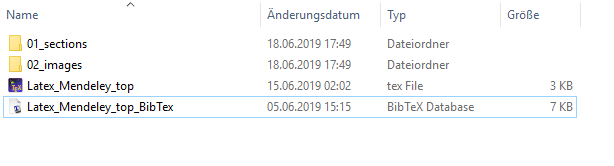
\includegraphics[width=1.0\textwidth]{02_images/latex_file_structure}
	\caption{Latex file structure used in this document.}
	\label{fig:latexfilestructure}
\end{figure}
